\section{Threads}\label{ch3}
In general, when we deal with parallel programs, the total CPU time spent by a parallel implementation is larger than a serial one, because parallelism involves an additional overhead caused by:

\begin{itemize}
    \item Synchronization and communication between threads;
    \item Exchange of data between threads;
    \item Load imbalance, i.e. threads that deal with smaller problems remain idle until other threads deal with bigger ones.
\end{itemize}

\subsection{Evaluation metrics}

Moreover, in general, evaluating a parallel algorithm is difficult, since its performances may depend on the architecture, on the network etc.. Some simple measures are:

\begin{itemize}
    \item The \textbf{parallel runtime $T_p(n)$}, where $p$ is the number of parallel units (cores), and $n$ is the problem size;
    \item The \textbf{cost $C_p(n) = pT_p(n)$}, which represents the total amount of work that is performed.
\end{itemize}

A parallel algorithm is said to be \textbf{cost optimal} if 

$$
C_p(n) = p T^*(n)
$$

, where $T^*(n)$ is the runtime of the fastest sequential algorithm for the given problem. In this sense, a parallel algorithm is cost-optimal if its cost has the same asymptotic growth as the fastest serial algorithm (as a function of the input size).

Another important metric for comparing sequential and parallel algorithms is the \textbf{speedup}, which is defined as:

$$
S_p(n) = \frac{T^*(n)}{T_p(n)}
$$

Theoretically, $S \leq p$, but in practice $S < p$, i.e. we have a \textit{sublinear speedup}, mainly due to the overheads we discussed before. Picture \ref{speedup} represents the speedup w.r.t to the number of processors.

\begin{figure}[h!]
		\centering
		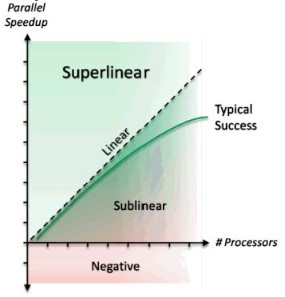
\includegraphics[scale = 1.5]{img/speedup.jpg}
        \label{speedup}
        \caption{Speedup vs number of processors}
\end{figure}

The goal when we implement a parallel algorithm is to measure a \textit{linear speedup}, i.e. $S = p$, and it is even possible to have \textit{superlinear speedup} because of cache sharing.

An alternative measure is \textbf{efficiency}:

$$
E_p(n) = \frac{S(n)}{p} = \frac{T^*(n)}{p T_p(n)}
$$

, and it is a measure of resource usage: it represents the fraction of time the processors are fully used to execute a fraction $1/p$ of the best sequential algorithm. We have that $E = 1$ for linear speedup.

When we deal with the evaluation of parallel algorithms, we have to consider two very important laws: the Amdahl's law and the Gustafson's law. The \textbf{Amdahl's law} regards speedup and says that the parallel execution time $T_p$ cannot be arbitrarily reduced by increasing $p$, i.e. the number of parallel units. If we suppose that a fraction $f$ of the computation cannot be executed in parallel (for example because of some dependencies), the have that:

$$
S_p(n) = \frac{T_{\text{seq}}}{T_{\text{par}}} = \frac{T_{\text{seq}}}{(f * T_{\text{seq}} + (1-f) * \frac{T_{\text{seq}}}{p})} = \frac{1}{f + \frac{1-f}{p}} \leq \frac{1}{f}
$$

, i.e. the sequential fraction $f$ is an upper bound of the speedup $S_p(n)$.

The \textbf{Gustafson's law} on the other hand regards scalability, and in particular it studies the behaviour of the algorithm when $n \to \infty$. In general, when we have a large amounts of data we would like to use a large number of processors. Suppose that the sequential part $c$ of an algorithm is constant w.r.t. to $n$. Then, let $T(n,p)$ be the execution time of the parallelizable part over $p$ processors: we define the \textbf{scaled speedup} as:

$$z
S_p(n) = \frac{c + T_1(n)}{c + T_p(n)} = \frac{c + T_1(n)}{c + \frac{T_1(n)}{p}} = \frac{\frac{c}{T_1(n)} + 1}{\frac{c}{T_1(n)} + \frac{1}{p}}
$$

When $n \to \infty$, we have:

$$
\lim_{n \to \infty} S_p(n) = p
$$

In general, the \textbf{scalability} of a parallel system is its ability to increase the speedup in proportion to the number of processors: scalable algorithms are characterized by a constant efficiency when increasing both the number of processors and the problem size.

\subsection{Shared-memory programming models}
\begin{itemize}
    \item \textbf{Process based models} assume that all data associated with a process is private by default, unless otherwise specified. Moreover, distinct page tables exist for each process in order to map the virtual addresses to distinct physical memory addresses. In this case, processes are units of resource ownership, i.e. they have their own program counter, heap memory etc.. Note that process can include more threads;
    \item \textbf{Thread based models} assume that all memory is global, i.e. the threads share the same address space (same page table), and there's at least one thread per process. Note that in this case the communication between the threads is far more easy than in the process based model;
    \item \textbf{Directive based models}: in this case the concurrency is specified in terms of high-level compiler directives, resulting in a sort of "annotated" source code. An example is given by the OpenMP library.
\end{itemize}

\subsection{pthreads}
In general, each thread has a separate execution flow, and it is the owner of a private program counter, stack memory, stack pointer etc.. , and they're also known as \textit{lightweight processes}. In this course we analyze the \textbf{pthreads} library (POSIX threads).

An example of the usage of the threads can be viewed in the matrix multiplication problem, as represented in Picture \ref{mm_threads}.

\begin{figure}[h!]
		\centering
		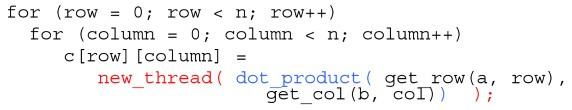
\includegraphics[scale = 1.5]{img/mm_threads.jpg}
        \label{mm_threads}
        \caption{Matrix multiplication with threads}
\end{figure}

In this case, we can consider a thread as the parallel asynchronous execution of a function with its parameters. In the \textit{pthreads} library, all the threads in a process are peers, and there's no explicit parent-child model, with the exception of the "main thread" that holds the process information. The main advantages over the processes are that threads can read/write to shared variables for communication, and that the context-switch operation is faster. The life cycle of a thread is represented in Picture \ref{threads}.

\begin{figure}[h!]
		\centering
		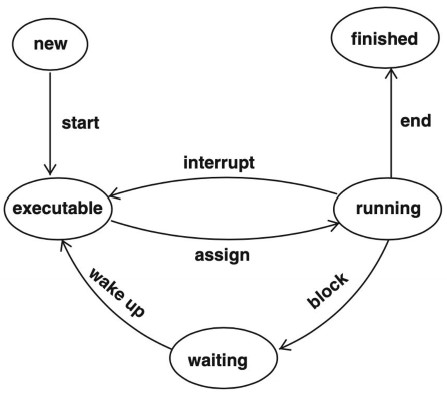
\includegraphics[scale = 1.5]{img/threads.jpg}
        \label{threads}
        \caption{Life cycle of a thread}
\end{figure}

An example of code that exploits the threads is shown in Picture \ref{pthreads example}.

\begin{figure}[h!]
		\centering
		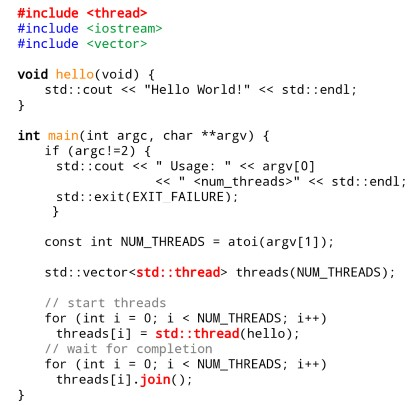
\includegraphics[scale = 1.7]{img/pthreads example.jpg}
        \label{pthreads example}
        \caption{Example of usage of threads}
\end{figure}

\begin{itemize}
    \item A vector of \textit{std::thread} objects is created. Notice that each thread object must be associated to a single actual thread;
    \item In the first for loop, each actual thread is created by passing the function \textit{hello}, which has no parameters;
    \item The second for loop is used to wait each thread to complete the execution, and this is done by the \textit{join} function.
\end{itemize}

In general, the class \textit{std::thread} is used to represent individual threads of execution: a thread is joinable, and it has a unique thread id. As we said before, a non-initialized thread does not represent a thread. The typical contructor for a thread is \textit{thread (function, arg1, arg2, .., argn)}, where the new thread of execution calls \textit{function} passing \textit{arg1, arg2, .., argn} as arguments. As we said before, no two \textit{std::threads} objects may represent the same thread of execution!

Other important functions are:

\begin{itemize}
    \item \textit{void join()}, which returns when the thread execution has completed, and after a call to this function, the thread object becomes non-joinable;
    \item \textit{void detach()}, which separates the thread of execution from the thread object, while the underlying thread executes independently;
    \item \textit{hardware\_concurrency()} returns the number of hardware thread contexts;
    \item \textit{void this\_thread::yield()}, which suggests the OS to re-schedule so as to allow other threads to be executed;
    \item \textit{void this\_thread::sleep\_for(duration)}, which stops the execution of the thread for duration, and the actual restart depends on OS scheduling decisions;
    \item \textit{void this\_thread\_sleep\_until(time\_point)}, which stops the execution until time\_point is reached. As before, the actual restart depends on OS scheduling decisions.
\end{itemize}

\colorbox{yellow}{\underline{Example}} (PI computation): the formula for deriving the value of $\pi$ can be approximated as:

$$
\pi = \frac{1}{n} \sum \limits_{i = 1}^n \frac{4}{1 + (\frac{i - 0.5}{n})^2}
$$

, the larger the $n$, the better the precision in the calculation of $\pi$. The idea to parallelize this computation is to split the work among the threads, in particular by assigning each thread a term of the summation, and then sum them up. Picture \ref{pi_function} shows the function that is called for each thread, while the others show the main.

\begin{figure}[h!]
		\centering
		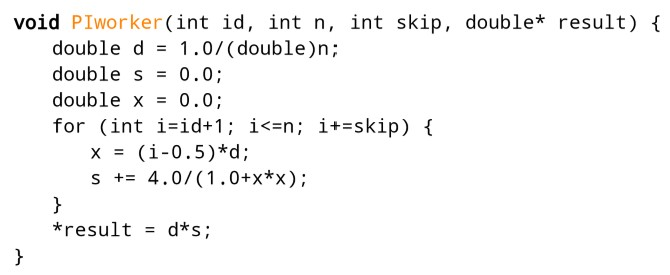
\includegraphics[scale = 1.4]{img/pi_thread.jpg}
        \label{pi_function}
        \caption{Function than computes the $\pi$}
\end{figure}

\begin{figure}[h!]
		\centering
		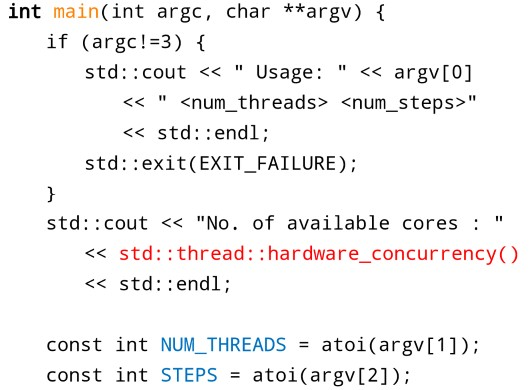
\includegraphics[scale = 0.8]{img/pi_main1.jpg}
        \label{pi_thread}
\end{figure}

\begin{figure}[h!]
		\centering
		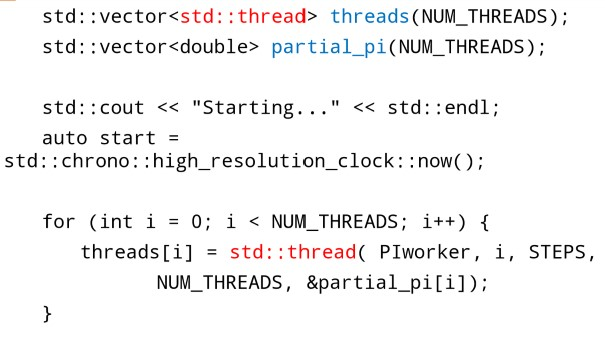
\includegraphics[scale = 0.8]{img/pi_main2.jpg}
        \label{pi_thread}
\end{figure}

\begin{figure}[h!]
		\centering
		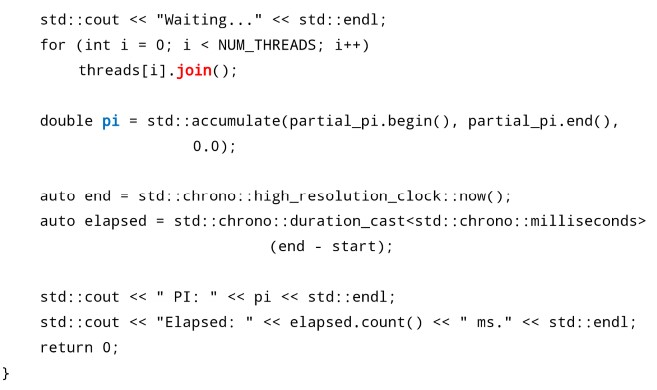
\includegraphics[scale = 0.8]{img/pi_main3.jpg}
        \label{pi_thread}
\end{figure}

As regards the \textit{PIworker} function:

\begin{itemize}
    \item the \textit{int skip} parameter determines the distance between the work of a thread and the work of another thread, since the work of the threads is interleaved;
    \item the result is stored into a variable, so it is not returned.
\end{itemize}

As regards the main:

\begin{itemize}
    \item we read from the terminal the number of threads and the value for the \textit{skip} parameter;
    \item a vector of threads is created: each thread writes in different part of the memory;
    \item a vector of double is created, to store the partial results.
\end{itemize}

\subsection{Mutex}
When multiple threads are manipulating the same data, results can be incoherent: we call \textit{critical section} the portion of code where a race condition occurs, and the idea of the \textit{mutual exclusion} is that at any point of time, only one thread can be in the critical section. In this sense, the \textit{mutex} is an object that prevents other threads with the same protection from executing concurrently and access the same memory locations. The main functions are:

\begin{itemize}
    \item \textit{void lock()}, to get the lock;
    \item \textit{void unlock()}, to release the lock;
    \item \textit{bool try\_lock()}, returns True if the lock was acquired;
    \item \textit{std::recursive\_mutex}, allows a thread to lock the same mutex multiple times;
    \item \textit{std::timed\_mutex}.
\end{itemize}

\colorbox{yellow}{\underline{Example}} (Consumer/Producer): the scheme of the consumer/producer problem is shown in Picture \ref{consumer_producer}. IN particular, the producer puts an item in the queue for 10 times, while the producer gets an item from the queue only it is not empty, again for 10 times. As we can see, the queue represents a critical section, since both the consumer and the producer access to it.

\begin{figure}[h!]
		\centering
		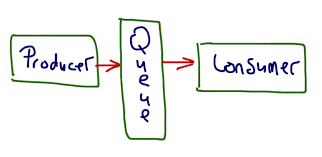
\includegraphics[scale = 0.8]{img/consumer producer.png}
        \label{consumer_producer}
        \caption{Consumer/Producer}
\end{figure}

Picture \ref{main} shows the main function to resolve the Consumer/Producer problem, while Picture \ref{consumer} and \ref{producer} shows the consumer and producer functions.

\begin{figure}[h!]
		\centering
		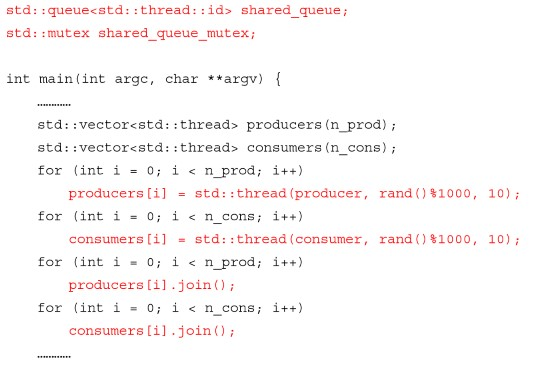
\includegraphics[scale = 1.4]{img/cp_main.jpg}
        \label{main}
\end{figure}

\begin{figure}[h!]
		\centering
		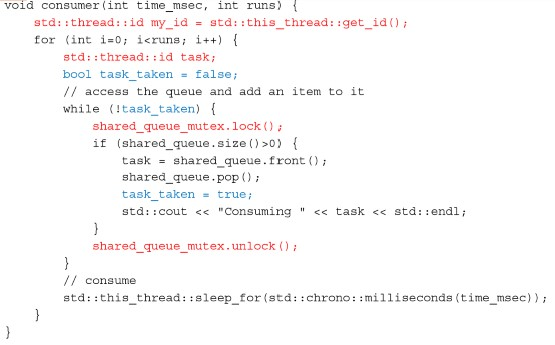
\includegraphics[scale = 1.4]{img/cp_c.jpg}
        \label{consumer}
\end{figure}

\begin{figure}[h!]
		\centering
		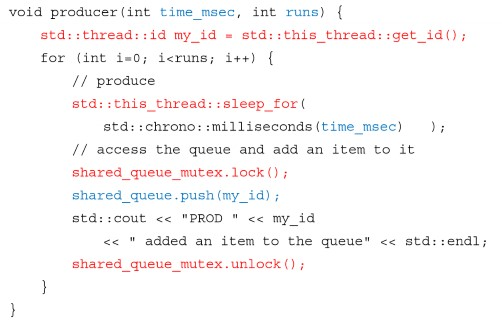
\includegraphics[scale = 1.4]{img/cp_p.jpg}
        \label{producer}
\end{figure}

For what regards the main:

\begin{itemize}
    \item we see that both a queue of thread IDs and a mutex are defined;
    \item a vector of threads is created, both for consumer and for producer: each consumer and each producer executes the respective function, then they're joined.
\end{itemize}

For what regards the producer, we see that before adding an item to the queue, the mutex is locked; then, after the writing, the mutex is unlocked, otherwise a deadlock would result. For what regards the consumer, we see that before reading the content of the queue, the mutex is locked, then if the queue is not empty, the value is read. Finally, the mutex is unlocked.

However, usually the mutexes are not used directly, but through:

\begin{itemize}
    \item \textit{lock\_guard(mutex)}, which allows to acquire a given mutex when created, and to release it when the end of the scope is reached;
    \item \textit{scoped\_lock}, which is similar to the previous one, but the locks are acquired and released on multiple mutexes.
\end{itemize}

, which allows easier handling and error free in case of exceptions or other issues. Moreover, the function \textit{std::call\_once(flag, callable, arg1..)} is used to make sure that a given function is executed only once even if invoked by multiple threads. The arguments are:

\begin{itemize}
    \item \textit{flag}, which should be an instance of \textit{std::once\_flag};
    \item \textit{callable}, which is a callable object, i.e. a function or anything supporting the () operator;
    \item \textit{arg1,..} are the arguments passed to the \textit{callable}.
\end{itemize}

Picture \ref{revised_producer} and \ref{revised_consumer} shows the revised implementation of the consumer and producer functions adopting the functions defined above.

\begin{figure}[h!]
		\centering
		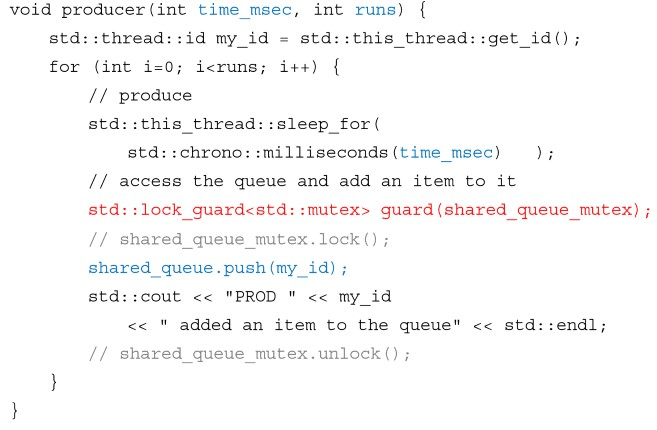
\includegraphics[scale = 1.4]{img/cp_revised_p.jpg}
        \label{revised_producer}
\end{figure}

\begin{figure}[h!]
		\centering
		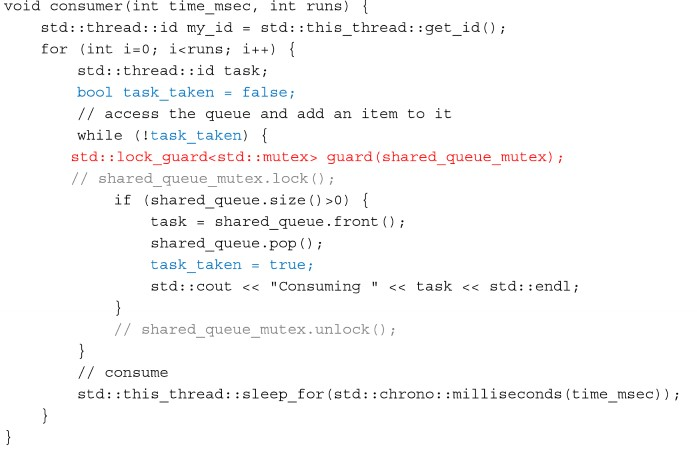
\includegraphics[scale = 1.4]{img/cp_revised_c.jpg}
        \label{revised_consumer}
\end{figure}

As we can see, the producer initialize a \textit{lock\_guard} passing the mutex as a parameter, and in this way the mutex is automatically locked and unlocked, so the \textit{lock()} and \textit{unlock()} functions are not needed anymore. On the other hand, the consumer does the same thing, so again the \textit{lock()} and \textit{unlock()} functions are not used.

Another useful tool that can be used are the \textbf{condition variables}, which allow a thread to block itself until specified data reaches a predefined state, which is checked by a predicate. In this sense, a condition variable can be thought as a notification system on the status of a variable, and it always has a mutex associated to it. The functioning is the following:

\begin{enumerate}
    \item A thread checks some data: if the data is ok it does some work, otherwise it waits;
    \item At some point the thread is awakened: it must re-check the data, since other threads may have been waiting for the same event and they may have already changed the status of the data.
    \item When a different thread modifies the data and reaches the desired status, it signals all the waiting threads.
\end{enumerate}

Notice that the shared data is accessed in mutual exclusion. If we consider the consumer/producer problem, we have:

\begin{itemize}
    \item the producer acquires a mutex, modifies the data and \textit{notify\_one} or \textit{notify\_all} on the condition variable, to wake up one or all threads on waiting;
    \item the consumer acquires s unique lock and executes the \textit{wait}, \textit{wait\_for} or \textit{wait\_until}. Then, the thread is awakened, it checks the condition and accesses the data.
\end{itemize}

Picture \ref{condition_p} and \ref{condition_c} shows the functions of the consumer and producer using the condition variable.

\begin{figure}[h!]
		\centering
		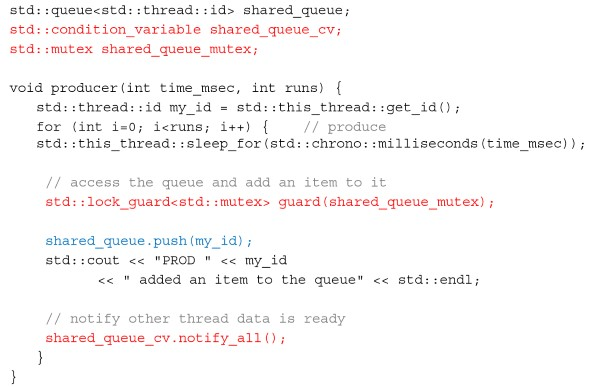
\includegraphics[scale = 1.4]{img/condition_p.jpg}
        \label{condition_p}
\end{figure}

\begin{figure}[h!]
		\centering
		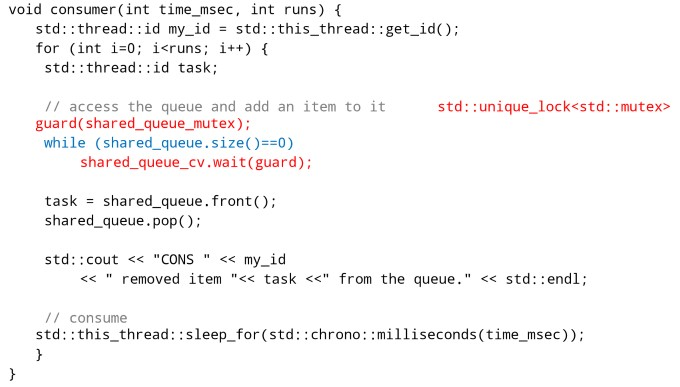
\includegraphics[scale = 1.4]{img/condition_c.jpg}
        \label{condition_c}
\end{figure}

As we can see, the condition variable \textit{shared\_queue\_cv} is created, and the producer notifies all the treads after writing in the queue. On the other hand, the consumer waits until the queue is not empty, and then it consumes the produced data. Notice that the while loop is very useful since many consumers may be waken up, so the loop is used to check whether some other consumer consumed the produced data. Moreover, we notice that the consumer waits on a unique lock.

Finally, other important tools are \textbf{atomic} and \textbf{promise/future}. The \textbf{atomic} creates a new variable whose modification and access does not cause data races. The \textbf{promise/future} tool allows to implement the communication between threads in a convenient way. An example is showed in Picture \ref{future_1} and \ref{future_2}.

\begin{figure}[h!]
		\centering
		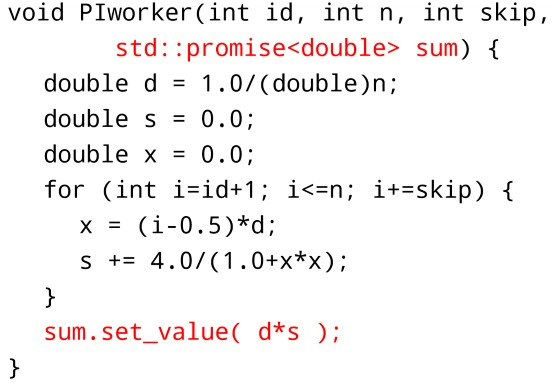
\includegraphics[scale = 1.4]{img/futures_pi.jpg}
        \label{future_1}
\end{figure}

\begin{figure}[h!]
		\centering
		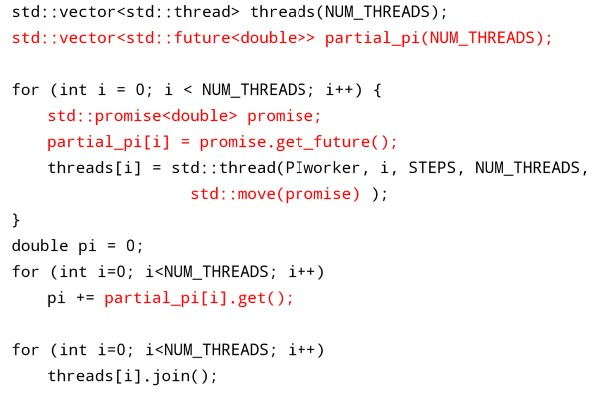
\includegraphics[scale = 1.4]{img/futures_pi_2.jpg}
        \label{future_2}
\end{figure}

Another way to launch a thread is by using the \textit{std::threads(std::launch policy, Function&& f, arg1,..)}, which runs the given function $f$ asynchronously and returns a \textit{std::future} that will eventually hold the result of that function call. The \textit{policy} can be:

\begin{itemize}
    \item \textit{async}, i.e. it creates a new thread that executes $f$ immediately;
    \item \textit{deferred}, i.e. the task is executed on the calling thread the first time its result (future) is requested
\end{itemize}

\subsection{OpenMP}
OpenMP is a very useful library for parallelizing some common patterns, e.g. for-loop, and it works by writing some instructions for the compiler, that automatically parallelizes the operations we indicate. In this sense, it provides the programmer a higher level of abstraction than pthreads, and it supports:

\begin{itemize}
    \item Parallel execution;
    \item Parallel loops;
    \item Critical sections;
    \item etc..
\end{itemize}

The OpenMP \textbf{directives} are based on the \textbf{\#pragma} compiler directives, and they consist of a directive name followed by some clauses, i.e. \textbf{\#pragma omp \textit{directive} [clause list]}. The OpenMP programs execute serially until they encounter the \textit{parallel} directive, which creates a team of threads that execute in parallel the given block. The main thread that encounters the parallel directive becomes the \textit{master} of the team of threads, and it is assigned with the thread id 0 within the group. We notice that despite executing in parallel the portion of code, no information is provided about the first thread that executes, the second etc.., i.e. the execution flow of each thread is not known.

\subsubsection{Basic clauses}
The \textbf{basic clauses} of the OpenMP library are:

\begin{itemize}
    \item \textit{num\_threads (int)}, that specifies the degree of concurrency, i.e. the number of threads that are created;
    \item \textit{if (scalar expression)}, that specifies the conditional parallelization, i.e. whether the parallel construct results in creation of not. If the expression evaluates false, the only one existing thread executes the following instruction block.
\end{itemize}

An example of the usage of this bases clauses is provided in Picture \ref{basis_clauses}.

\begin{figure}[h!]
		\centering
		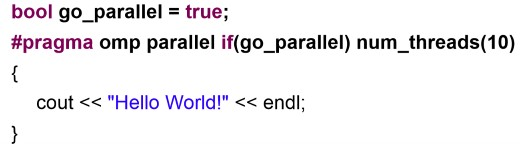
\includegraphics[scale = 1.4]{img/basis clauses.jpg}
        \label{basis_clauses}
\end{figure}

\subsubsection{Variable sharing clauses}
In OpenMP we can specify the level at which the variables of the code are shared among the threads that are created (in the following list, $x$ refers to a variable outside the block which can be accessed by the threads):

\begin{itemize}
    \item \textbf{private(x)}: in this case each thread has his own copy of $x$; $x$ is not initialized, so its initial value is undefined;
    \item \textbf{shared(x)}: in this case every thread accesses the same memory location, so it introduces race condition;
    \item \textbf{firstprivate(x)}: in this case each thread has his own copy of $x$, and $x$ is initialized with the current value of $x$ before the various threads start;
    \item \textbf{default (shared/none)}: affects all the variables not specified in other clauses
\end{itemize}

An example of the functioning of these clauses is provide in Picture \ref{variable_sharing}: as we can see, the number of threads is 10, and the variable $a$ is accessed as private, $b$ and $d$ are shared, while $c$ is firstprivate. In this sense, we see that the value of $a$ and $c$ at the end of the block are 1, since the increments are done in the private copies of the threads, while the values of $b$ and $d$ are 11, since they're incremented by each of the 10 threads.

\begin{figure}[h!]
		\centering
		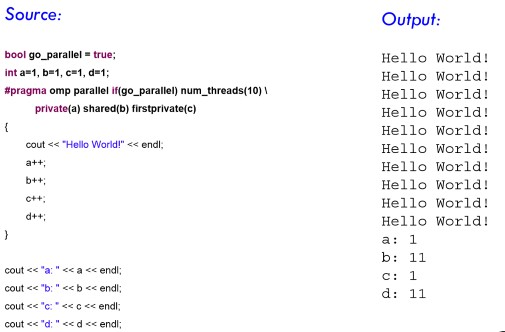
\includegraphics[scale = 1.6]{img/variable sharing clauses.jpg}
        \label{variable_sharing}
\end{figure}

It is important to notice that there's no guarantee that for the \textit{shared} variables the increments are atomic, so the result of the previous code could also be different from 11 in some cases, due to the race condition described above.

\subsubsection{Reduction clause}
The \textbf{reduction clause} specifies how multiple \textbf{local copies} of a variable at different threads are \textbf{combined} into a single copy at the master when threads exit. The clause is defined as \textit{reduction (operator: variable list)}, where:

\begin{itemize}
    \item each variable of the list is accessed as \textit{private} by each thread, and the variable is initialized as the value which is neutral w.r.t. the \textit{operator} (if +, then it is initialized as 0, if * as 1 etc..);
    \item the \textit{operator} can be one of +, *, -, &, |, etc..
\end{itemize}

An example of the functioning of reduction clause is provided in Picture \ref{reduction_clauses}. As we can see, $b$, $c$ and $d$ are shared, so their values are 11, while the value of $a$ is incremented in each thread to 2, then it is reduced using the * operator, so the overall computation is $2*2*..*2 = 2^{10} = 1024$.

\begin{figure}[h!]
		\centering
		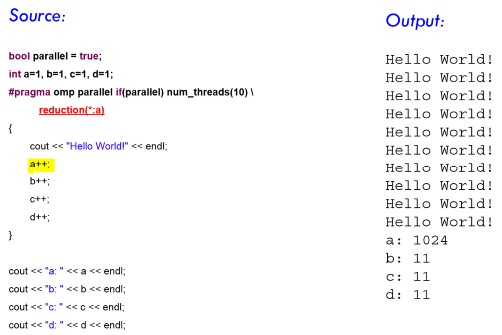
\includegraphics[scale = 1.6]{img/reduction clauses.jpg}
        \label{reduction_clauses}
\end{figure}

\subsubsection{\textit{for} directive}
OpenMP provides a directive \textit{for} to split iterations of the subsequent for loop among available threads: an example is provided in Picture \ref{for_clause}. As we can see, the code computes the sum of the first 10 squared numbers, and the variable \textit{add} is reduces according to the operator +.

\begin{figure}[h!]
		\centering
		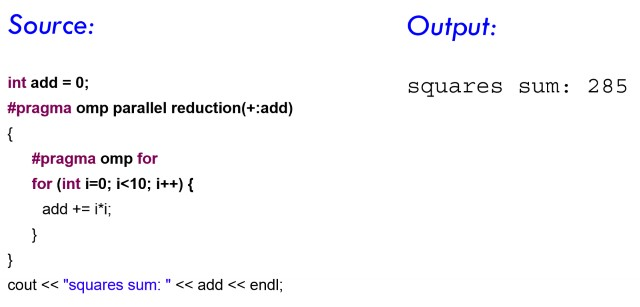
\includegraphics[scale = 1.6]{img/for clause.jpg}
        \label{for_clause}
\end{figure}

An additional clause can be attached to the \textit{for} directive, and it is the \textit{schedule} clause. The \textit{schedule}  is defined as \textit{schedule (policy [, param])}, and it deals with the assignment of iterations to each thread. The policies can be:

\begin{itemize}
    \item \textbf{schedule(static)}: in this case the loop is statically split into chunks and each chunk is statically assigned to a thread. Notice that we still do not know in which order the chunks will be executed;
    \item \textbf{schedule(dynamic)}: in this case the loop is statically split into chunks, and each thread asks for the next chunk to be executed. We do not know how much chunks each thread will execute, but this policy is useful to balance the load;
    \item \textbf{schedule(guided)}: in this case the chunk size decreases exponentially in time. Long tasks are assigned soon to minimize any overhead, while short tasks are assigned at the end to avoid idle threads and to have threads that complete their chunks at the same time;
    \item the \textit{param} specifies the chunk size; if the policy is \textit{guided}, then it specifies the minimum chunk size.
\end{itemize}

Other additional clauses are the \textit{nowait} clause and the \textit{ordered} directive. The \textit{nowait} clause enables the thread that completed the for loop execution to proceed the parallel execution of the rest of the code, while the \textit{ordered} directive forces a piece of code to be executed according to the natural order of the for loop. 

Finally, there are some restrictions in order to apply the \textit{for} directive:

\begin{itemize}
    \item for loops must not have break statements;
    \item loop control variable must be integer, as its initialization expression;
    \item the logical expression must be of $<, \leq, > , \geq$;
    \item the increments/decrements must have integers.
\end{itemize}

\subsubsection{Sections}
OpenMP supports non-iterative parallel task assignment using the \textit{sections} directive: in this case, each section is executed by only one thread (in parallel). There exist some synchronization directives:

\begin{itemize}
    \item \textbf{barrier}: all the threads must wait for each other to reach the barrier;
    \item \textbf{single[nowait]}: the following structures block enclosed is executed by only one thread in the team. Threads in the team that are not executing the single single block have to wait at the end of the block unless \textit{nowait} is specified;
    \item \textbf{master}: only the master thread of the team executes the block enclosed by this directive, the others skip it and continue;
    \item \textbf{atomic}, which ensures atomicity of expressions like $x++, ++x, x--, --x$ etc..;
    \item \textbf{critical[(name)]}, which restricts access to the structured block to only one thread at a time. The optional name argument identifies the critical region: no two threads can enter the critical section with the same name.
\end{itemize}

\subsubsection{Synchronization issues}
OpenMP is able to synchronize shared variable, but the \textbf{compiler} may unpredictably optimize the code, and in general it uses a minimum effort approach on synchronization. The \textit{flush(var list)} directive can be used to synchronize a set of shared variables among the threads in the team.

\subsubsection{OpenMP vs explicit thread management}
\begin{itemize}
    \item Directives layered on top of threads \textbf{facilitate a variety of
    thread-related tasks}, and the programmer is \textbf{rid of the tasks} of initializing attributes objects, setting up arguments to threads, partitioning iteration spaces, etc..;
    \item However, using explicit threading the \textbf{data exchange is more apparent}, and this helps in alleviating some of the overheads from data movement, false sharing, and contention. Explicit threading also provides a \textbf{richer API} in the form of condition waits, locks of different types, and increased flexibility for building composite synchronization operations;
    \item Finally, since explicit threading is used more widely than OpenMP, \textbf{tools and support} for Pthreads programs are \textbf{easier} to find.
\end{itemize}

\colorbox{yellow}{\underline{Example}} ($\pi$ computation): Picture \ref{pi_computation} shows the code for the parallel computation of $\pi$. We recall that the formula is 

$$
\pi = \frac{1}{n} \sum \limits_{i = 1}^n \frac{4}{1 + (\frac{i - 0.5}{n})^2}
$$

Some comments:

\begin{itemize}
    \item we see that the \textit{parallel} and \textit{for} directive are put together;
    \item the variable \textit{pi} is reduced using the + operator (see the formula);
    \item $x$ and $d$ are private, and $d$ is initialized as $\frac{1}{n}$
\end{itemize}

\begin{figure}[h!]
		\centering
		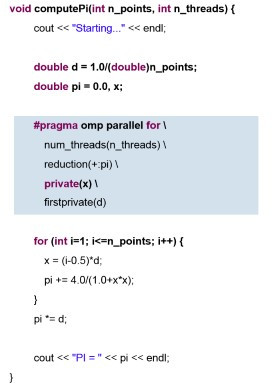
\includegraphics[scale = 1.8]{img/pi computation.jpg}
        \label{pi_computation}
\end{figure}


\colorbox{yellow}{\underline{Example}} (Mandelbrot set): the Mandelbrot set is the set $c$ of complex numbers such that the following function does not diverge:

$$
\begin{cases}
	z_0 = 0 \\
	z_{k + 1} = z_k^2 + c
\end{cases}
$$

The issues about this example are that the number of iterations $k$ is unknown, and the overall computation could lead to potential load imbalance, i.e. it can create very short or very long tasks! Picture \ref{mandelbrot} shows the parallel computation of the Mandelbrot set.

\begin{figure}[h!]
		\centering
		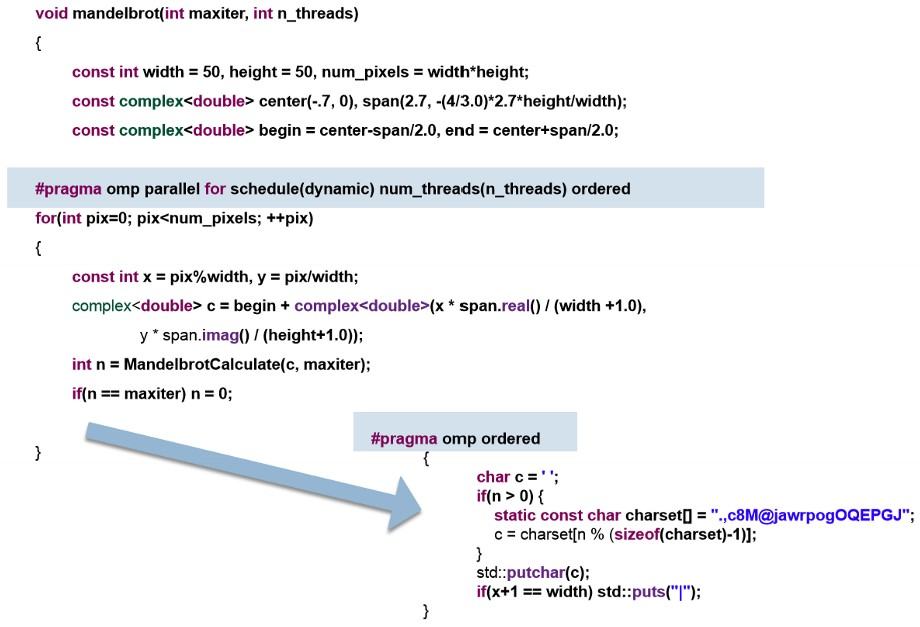
\includegraphics[scale = 1.6]{img/mandelbrot.jpg}
        \label{mandelbrot}
\end{figure}

As we can see:

\begin{itemize}
    \item the schedule is \textit{dynamic}, since the function could have some load imbalance;
    \item the \textit{ordered} directive is used for the output of the points, since we have some constraints in their order.
\end{itemize}


\subsection{OpenMP and Cache}
Once we introduced the OpenMP library, we can now analyze in detail some of its results when used for solving some classic problems. For example, if we consider again the \textbf{matrix multiplication problem}, we can compare the sequential and the parallel computation.

If we consider the sequential computation, showed in Picture \ref{sequential}, we see that each of the three for loops can be parallelized.

\begin{figure}[h!]
		\centering
		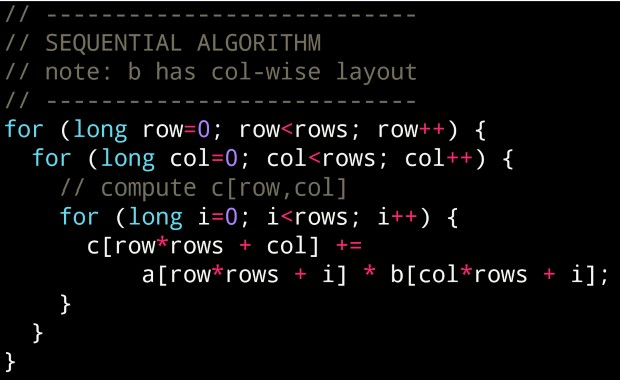
\includegraphics[scale = 1.6]{img/sequential.jpg}
        \label{sequential}
        \caption{Sequential algorithm}
\end{figure}

Intuitively, if we parallelize the most external loop, then $10$ threads are created; if we parallelize the central loop, then $10$ threads are created for each external loop, so $10*N$ threads, where $N$ is the number of rows; finally, if we parallelize the most internal loop, $10*N^2$ threads are created. 

More specifically, by parallelizing the external loop, a thread is created for each row of the matrix $A$, and it scans the full $B$ before writng a new row in $C$: from the point of view of the cache this is quite bad, since the matrix $B$ usually does not fit entirely in the memory. 

On the other hand, if we parallelize the central loop, a thread is created for each column of matrix $B$, and it writes a column in $C$. The advantages of this approach are:

\begin{itemize}
    \item differently from the previous case, not the entire matrix $A$ needs to be stored in memory, but only one row, since all the threads will access the same row for computing a column of $C$. Thus, this approach is very nice since it is characterized by a great cache locality;
    \item each thread computes one column at at time, so we only need to store one column for each thread, which is better for the cache.
\end{itemize}

On the other hand, the main disadvantage of this approach is that the threads are created and destroyed multiple times, resulting in a quite high overhead. Finally, the last approach is to parallelize the internal loop: the code is provided in Picture \ref{par3}.

\begin{figure}[h!]
		\centering
		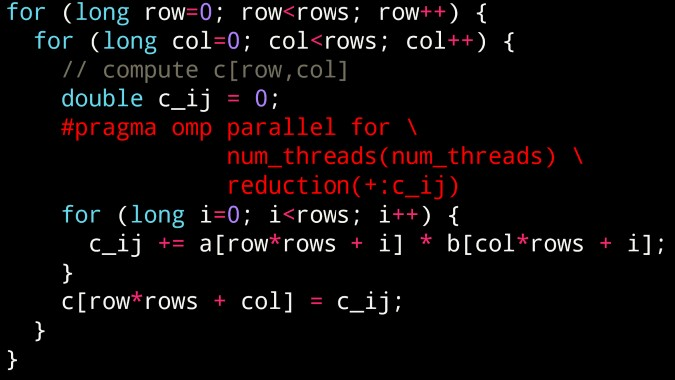
\includegraphics[scale = 1.6]{img/par3.jpg}
        \label{par3}
        \caption{Parallel algorithm: third strategy}
\end{figure}

As we can see, the count variable $c_{ij}$ is used to store the partial sums, and it is updated by each thread independently. In this sense, the parallelization is applied at single row and single column level. From the point of view of the cache, we only need to store one row and one column at a time, and this is very nice, but on the other hand the threads are created and destroyed $N^2$ times, so there's a huge overhead due to thread management.

The resulting execution times were:

\begin{itemize}
    \item 11,500ms for the sequential computation;
    \item 800-1,200ms for the first version of the parallel computation;
    \item 700-6,000ms for the second version of the parallel computation;
    \item 153,923ms for the last version of the parallel computation.
\end{itemize}

In general, we notice a sort of \textbf{instability} in the timings, and this phenomenon is due to the fact that threads can be rescheduled to a different core/processor, and in this case the thread is moved to a different core (or CPU) along with all the data. This phenomenon leads to many cache misses and to a significant decay of the performances, and it can be solved by forcing the threads to not move along the cores, by using the command \textit{export OMP\_PROC\_BIND = true}.

However, we notice that the second strategy is the one that better performs for our task. Now the goal is to \textbf{reduce the thread management overhead}, since, as we underlined before, the threads are created and destroyed multiple times (in particular, once for each row). A solution for this problem is given by switching the first and the second loop: in this case, each thread of the column is destroyed after all the rows of $A$ are scanned, but in terms of the cache this is worse, since we need now to store the matrix $A$ entirely. The code is showed in Picture \ref{par4}.

\begin{figure}[h!]
		\centering
		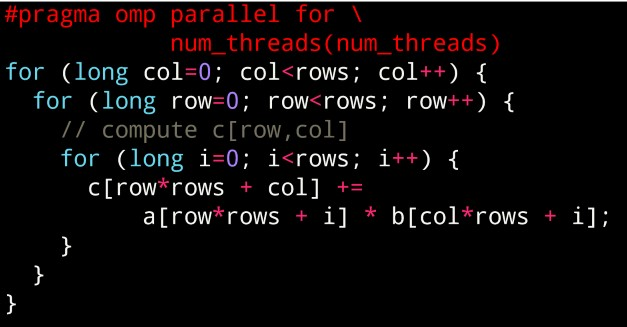
\includegraphics[scale = 1.6]{img/par4.jpg}
        \label{par4}
        \caption{Parallel algorithm: inverted strategy}
\end{figure}

A possible improvement to this implementation is showed in Picture \ref{par5}.

\begin{figure}[h!]
		\centering
		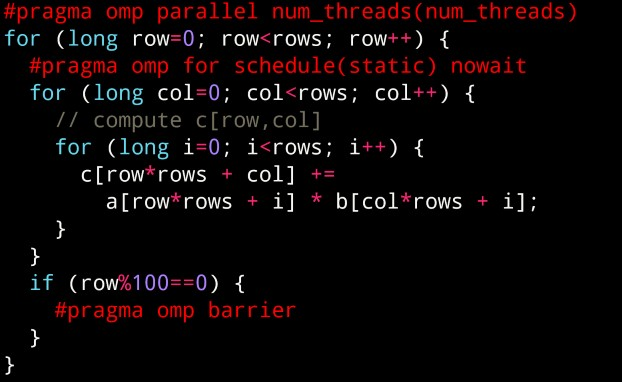
\includegraphics[scale = 1.6]{img/par5.jpg}
        \label{par5}
        \caption{Parallel algorithm: synchronized strategy}
\end{figure}

As we can see, first of all the loop is statically split into chunks, and the \textit{nowait} directive means that once a thread has completed the row, it moves to the following one, resulting in an increased number of rows that are processed simultaneously. Moreover, this approach results in less synchronization overhead and, potentially, in a better use of the cache; however, on the other hand, this reduction of synchronization could result in no cooperation between threads (so in less cache hits) and could lead to situations in which the data do not fit into the cache. For these reasons, a thread synchronization is performed after 100 rows of $A$ (note that this quantity depends on the cache memory that is available).

The timings for the strategy we described above are:

\begin{itemize}
    \item 810ms for the inverted strategy;
    \item 348ms for the synchronized strategy.
\end{itemize}

In particular, recalling that the time for the sequential implementation was 11,500ms, we notice that using the synchronized strategy we reach a speedup of $\frac{11,500}{348} = 33$, which is a great result.

\subsection{\textit{perf}}
The Linux OS provides the \textit{perf} command for profiling the execution of a given program, and in particular it allows to measure the number of misses for each level of the cache, the percentage of misses etc..
